\section{Overview}



\subsection{Original Design, Performance}

The CLAS Cherenkov detector~\cite{Adams:2001kk} has been instrumental in identifying the electrons during the CLAS6 era.
It provided eletrons/pions discrimination with $~90\%$ efficiency.

It consists of six identical sectors, each containing:

\begin{itemize}
	\item 108 Lightway adjustable mirrors
	\item 36 Winston light collecting Cones
	\item 36 5" Photonis X4500B PMT
	\item 36 Magnetic Shields
	\item C4F10 Gas, refraction index: 1.00134
\end{itemize}


The optics of each module is designed to focus the light onto a photomultiplier tube (PMT) associated with that module and located in the region obscured by the coils.
Fig.~\ref{fig:optics} shows the optical arrangement of one module. The array of the modules in one sector is shown in Fig.~\ref{fig:ltccArray}.

\begin{figure}[hbt]
	\centering
	\includegraphics[width=1.0\columnwidth,keepaspectratio]{img/optics.png}
	\caption{Optical arrangement of one of the 216 optical modules of the CLAS Cherenkov detector, showing the optical and light collection components.}
	\label{fig:optics}
\end{figure}

\begin{figure}[hbt]
	\centering
	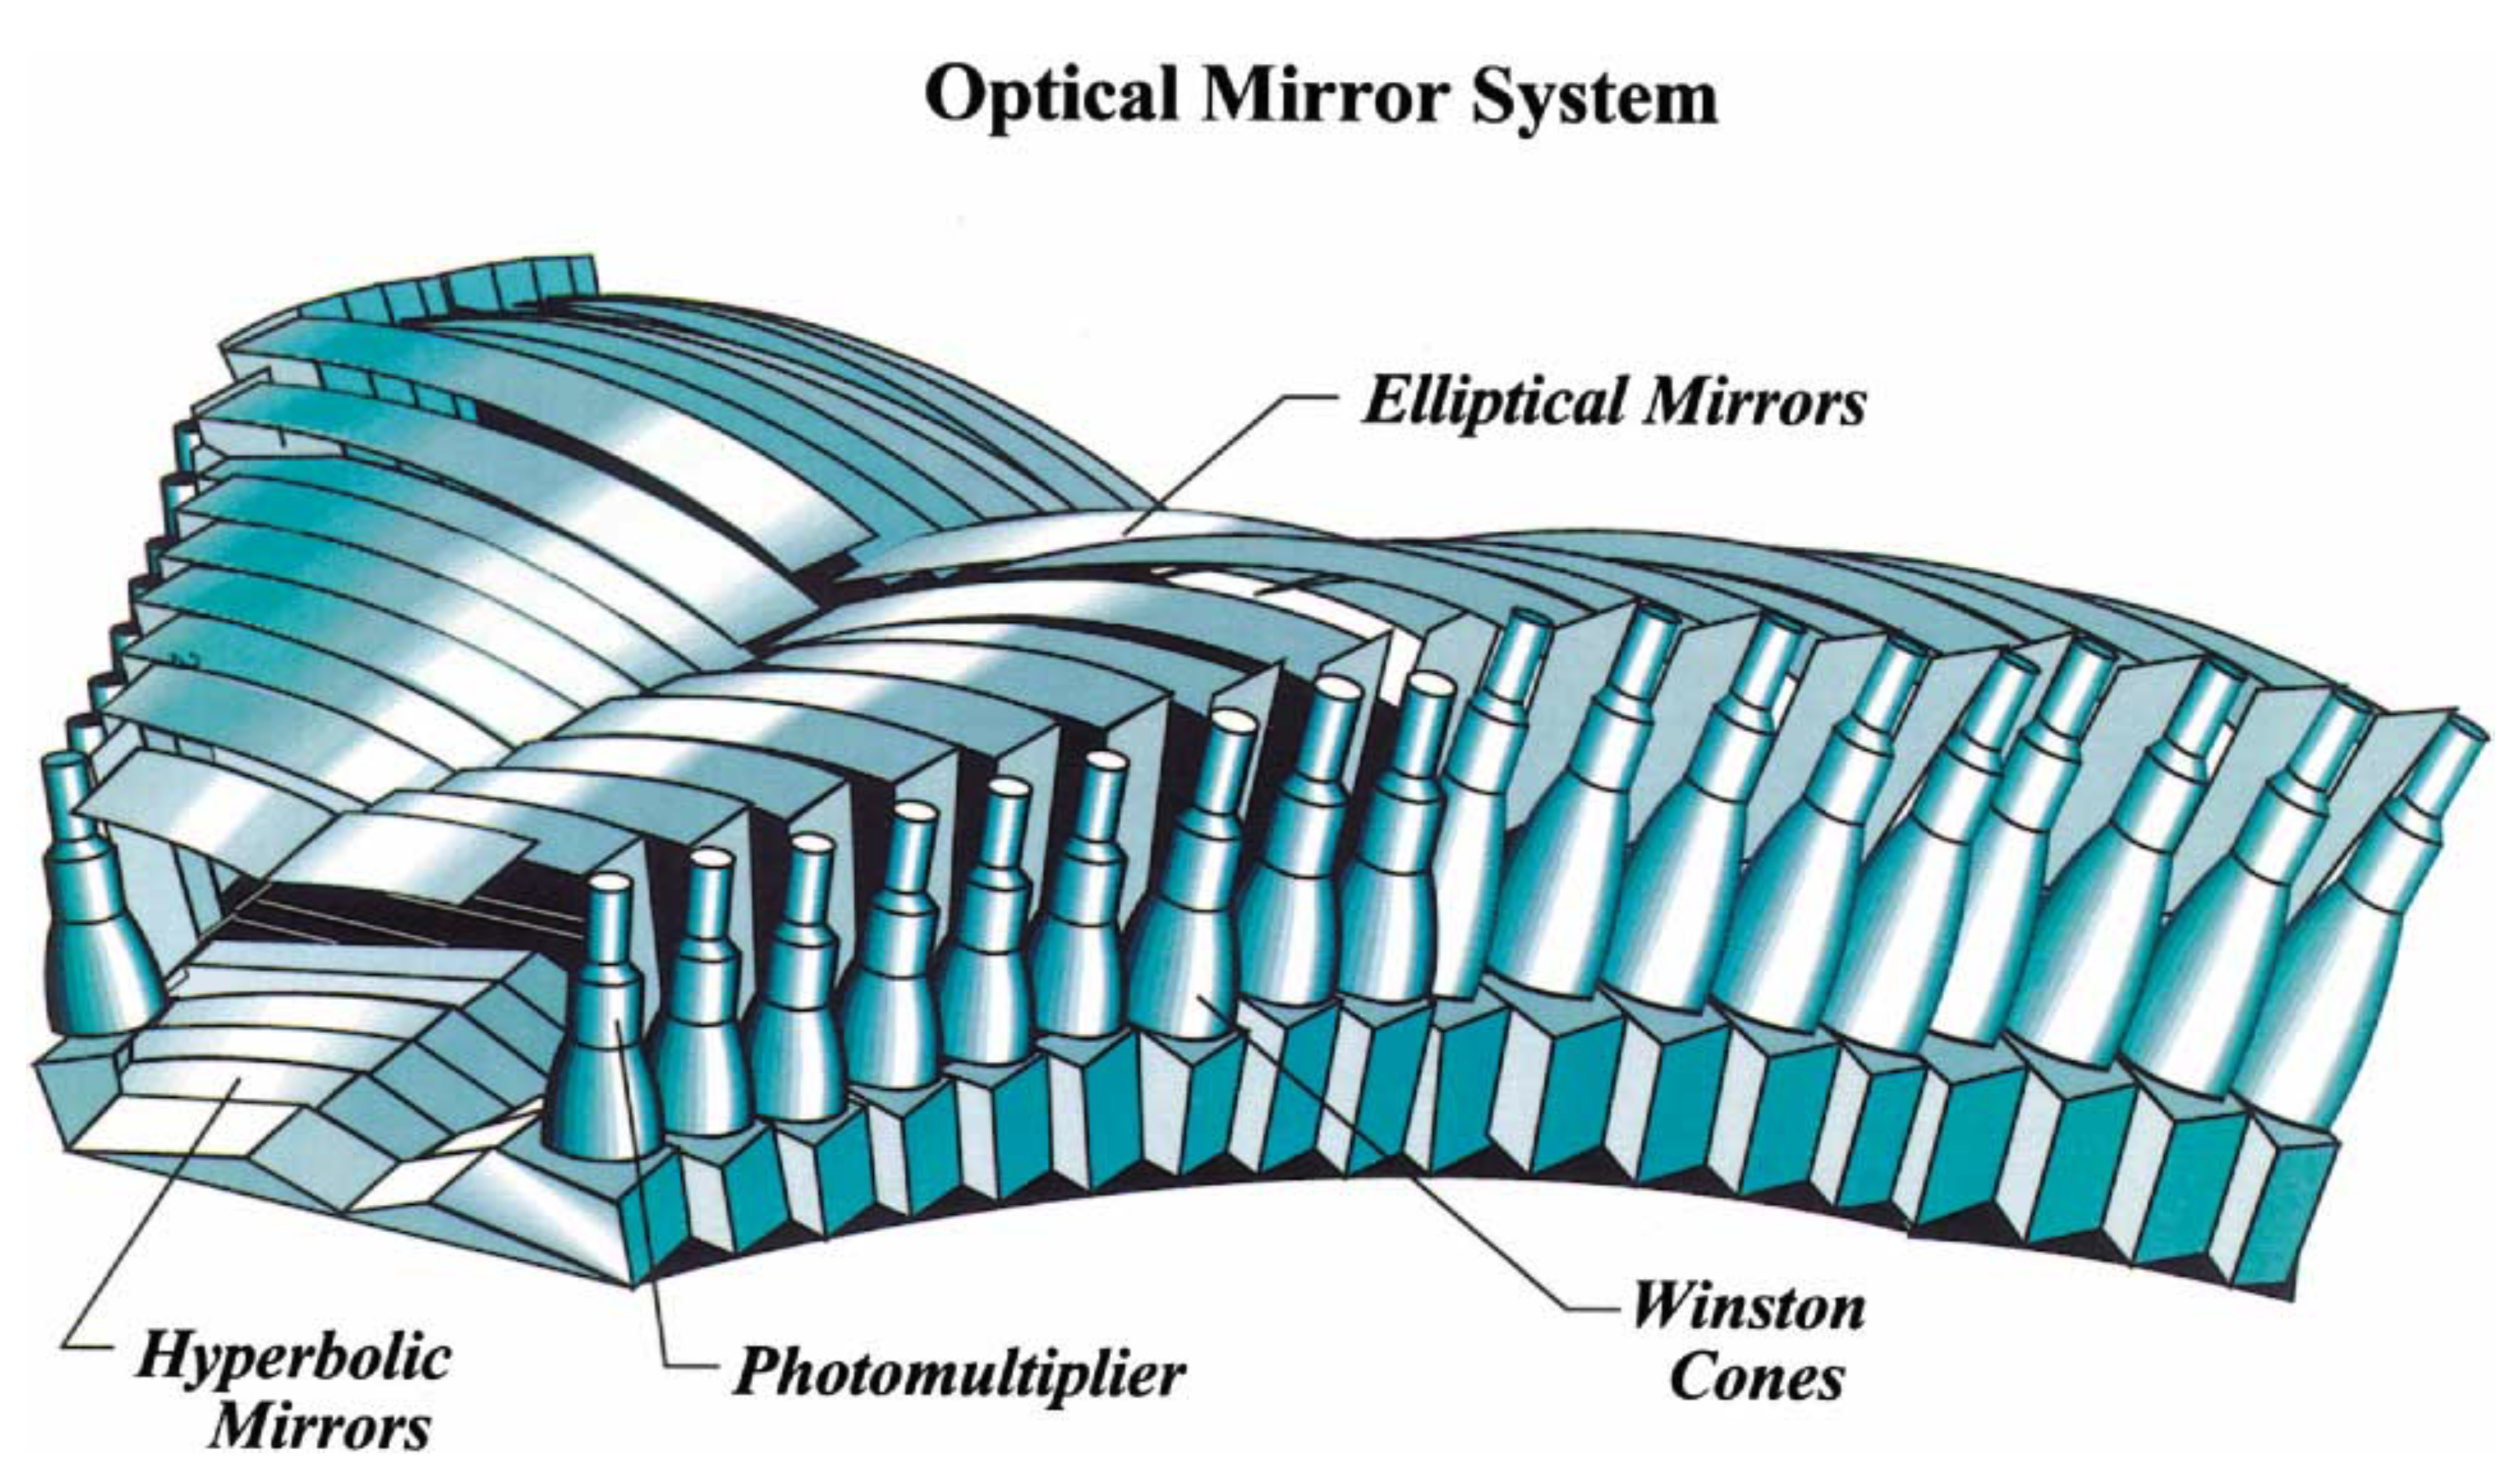
\includegraphics[width=1.0\columnwidth,keepaspectratio]{img/ltccArray.png}
	\caption{A schematic diagram of the array of optical modules in one of the six sectors.}
	\label{fig:ltccArray}
\end{figure}

The detector was operational for about $17$ years. The typical number of photo-electrons detected, coming from electrons, was between 10 and 20.
The PMT gain needed $x10$ multiplier electronics to be digitized by the ADCs and TDCs.

The detector had a few malfunctions: it was leaking gas at a rate of about $\$50K$ / year, the mirrors alignment had inefficiencies that affected
the signal strength and the mirrors support broke in all sectors.


\subsection{Upgrade}

With the higher beam energy of the upgraded accelerator~\cite{TDR12} the momentum of the particles increases substantially.
Given the pion Cherenkov threshold of $2.6$ GeV/c, the detector cannot provide a good electron/pion discrimination for most energies and a new
High Threshold Cherenkov Counter (HTCC) with a $CO_2$ gas sytem has been built to provide electron discrimination up to momenta of $~6 GeV/c$.

The heavier $C_4F_{10}$ gas can still be used to discriminate pions from kaons, see Fig.~\ref{fig:newScope} thus the detector was refusbished
to a Low Threshold Cherenkov Counter (LTCC).

The box has been modified so the

\begin{itemize}
	\item Support the new scope of pion/kaon discrimination
	\item Address the gas leaks and other hardware inefficiencies.
\end{itemize}

\begin{figure}[hbt]
	\centering
	\includegraphics[width=1.0\columnwidth,keepaspectratio]{img/newScope.png}
	\caption{With the accelerator and CLAS12 upgrade, the momentum range of the detected particles has been extended significantly. While the HTCC
            provides the new electron/pion identification, the LTCC has been refusbished to provide a pion/kaon discrimination.}
	\label{fig:newScope}
\end{figure}
